\documentclass[11pt]{article}
\usepackage[preprint]{acl}
\usepackage{times}
\usepackage{latexsym}
\usepackage[T1]{fontenc}
\usepackage{amsmath}
\usepackage[utf8]{inputenc}
\usepackage{microtype}
\usepackage{inconsolata}
\usepackage{graphicx}
\usepackage{booktabs}
\usepackage{amssymb,tabularx}
\title{A Lightweight Noise Filter for Distant Supervision\\
\large Learned Rule Weights and Clean-Data Retention}
\author{
  Zijun Wu \quad Tianchen Xie \quad Tianluo Zhang\\
  New York University\\
  New York, USA\\
  \texttt{\{zw4238, tx813, tz2668\}@nyu.edu}
}
\begin{document}
\maketitle
\begin{abstract}

A filter can achieve high noise recall by discarding most of its useful supervision. We revisit a hand-written linguistic filter and compare six lightweight models under an explicit clean-retention objective. A sparse L2 logistic model combines the original rules with entity-masked local words and bigrams, candidate-relation indicators, and relation-feature interactions. Five-fold nested sentence-grouped evaluation on 4,241 labeled development examples yields 89.93\% clean retention and 31.84\% noise recall, compared with 90.94\% and 19.58\% for a rule-feature logistic baseline. On 3,966 diagnostic test examples without development-sentence overlap, the new model retains 92.37\% of clean examples and removes 30.44\% of noise. A separate, smaller noise-focused diagnostic does not show the same improvement. The evidence supports a better measured retention-quality trade-off, not a neural benchmark win or a downstream relation-extraction claim.

\end{abstract}

\section{Introduction}

Distant supervision aligns knowledge-base facts with text to obtain relation-extraction training data without labeling every sentence \citep{mintz-etal-2009-distant}. The task here is to decide whether a supplied relation label is supported by a sentence mentioning two entities. An incorrect NA label is also noise: NA does not automatically mean an example is useless. We therefore evaluate both NA and non-NA examples and select separate operating thresholds for these groups.

The previous recall-first objective encouraged removal of roughly 90\% of labeled noise even when correct examples were also removed. This release separates two questions: does a model rank label validity better, and which operating point preserves useful data? Lowering the removal rate alone is not evidence of a better model.

We investigate the progression from linguistic hypotheses to learned rule weights and contextual evidence. Our contribution is a controlled comparison of six CPU-only filters with explicit retention objectives, grouped validation, and diagnostic failure analysis.
\section{Related Work}
\paragraph{Distant supervision and instance selection.}
\citet{mintz-etal-2009-distant} use knowledge-base relations to supervise extraction from text. The distinction between a relation holding for two entities and that relation being expressed in a particular sentence motivates the latent mention-level decisions of \citet{riedel2010modeling}. Our filtering task similarly evaluates a supplied label for an individual sentence and entity pair.

Selective attention aggregates useful evidence within entity-pair bags \citep{lin-etal-2016-neural}. ARNOR regularizes attention toward relation patterns and selects trustworthy instances \citep{jia-etal-2019-arnor}. These approaches motivate examining the evidence supporting each label. We retain ARNOR's version-2 corpus as the data source, while using inspectable linguistic and lexical features rather than a neural attention encoder.

\paragraph{Additional supervision and structured knowledge.}
\citet{beltagy-etal-2019-combining} combine distant and direct supervision, using directly supervised examples to improve attention-based noise identification. This distinction is relevant to our progression from a training-free rule scorer to logistic weights fitted using validity annotations: the learned model has access to additional supervision.

CoType jointly represents entity mentions, relation mentions, features, and type labels, incorporating a partial-label objective for noisy supervision \citep{ren2017cotype}. Knowledge-attention incorporates external lexical knowledge into neural relation extraction \citep{li-etal-2019-improving}. Our relation-conditioned rules and local context also distinguish evidence by the candidate relation, but do not reproduce these joint embedding or attention architectures.

\paragraph{Data construction and evaluation scope.}
\citet{shah-etal-2022-enhanced} introduce state-change information into distant-supervision data construction to reduce noise. Such curation complements the post hoc filtering studied here. Our controlled comparisons concern lightweight validity filters; the published relation-extraction scores of the above systems are not interchangeable with our binary noise-detection metrics. We do not present them as directly evaluated baselines.

\section{Method}
\subsection{Linguistic rules and learned weights}

Hand-written rules score entity distance, intervening-text length, relation keywords, and entity order, and penalize uncertainty, list-like text, and overlapping entities. Rule-feature logistic regression learns how to combine eight such components and an NA indicator. The new sparse model additionally conditions on the candidate relation, learns relation-specific rule weights, and reads entity-masked local unigrams and bigrams. Its coefficients remain inspectable; no pretrained encoder or GPU is required.



For a sentence $s$, entity mentions $h,t$, and candidate relation $r$, let $y=1$ denote an unsupported label. The original rules produce a vector $q(s,h,t,r)\in\mathbb{R}^{8}$. A hand-weighted score combines these components; the learned baseline instead estimates
\begin{equation}
p_\theta(y=1\mid x)=\sigma\bigl(w^\top\phi(x)+b\bigr),
\end{equation}
where $\phi$ contains the rule components and an NA indicator. We fit L2-regularized logistic regression and select its inverse regularization parameter on inner validation folds.
\subsection{Relation-conditioned local context}
The full representation adds candidate-relation indicators, interactions between relation and rule features, and binary unigram/bigram indicators with their relation interactions. Entity names are replaced by head/tail markers. Context includes up to four tokens before and after the entity pair and the intervening text; when the latter exceeds 40 tokens, its first and last 20 tokens are retained with a gap marker. Local and intervening-text features are encoded separately. These choices restrict feature growth and avoid directly exposing entity names.
\subsection{Retention-aware decisions}
An example is removed when its score meets or exceeds a threshold $\tau_g$, where $g$ distinguishes NA and non-NA candidates. Retain90 selects
\begin{equation}
\tau_g^*\in\arg\max_{\tau}\widehat{R}_{\rm noise,g}(\tau)
\end{equation}\begin{equation}\text{subject to}\quad\widehat{R}_{\rm clean,g}(\tau)\geq0.90.
\end{equation}
The constraint is fitted on inner predictions and is not a population guarantee. Retain95 increases the target to 0.95; Recall90 reverses the roles, maximizing clean retention subject to a noise-recall target of 0.90.
\section{Experimental Setup}

Data: the authors' ARNOR 2.0 corpus. This release is a supervised validity-filter experiment using labeled development data; it is not a reimplementation of ARNOR's distant-supervision training protocol. All files are identified by SHA-256 in configs/data\_manifest.json. Raw news articles are not redistributed.

\begin{table*}[t]\centering\small
\resizebox{\textwidth}{!}{\begin{tabular}{@{}lrrrr@{}}\toprule
Split & Raw mentions & Valid labeled, unique & Sentence groups & After dev-text exclusion\\\midrule
Development & 4567 & 4241 & 1495 & -\\
Test & 4484 & 4050 & 1486 & 3966\\
Noise-focused test & 533 & 301 & 157 & 297\\
\bottomrule\end{tabular}}
\caption{Corpus audit and evaluation populations.}
\end{table*}

Entity spans must resolve uniquely and match the text. We quarantine 326 development, 425 test, and 200 noise-focused mentions with ambiguous spans. We remove 9 duplicate test annotations and 26 duplicate noise-focused annotations; 4 unknown and 2 conflicting noise-focused labels are excluded. Counts are disclosed rather than silently treated as clean. Production inference emits an explicit abstention for uncertain spans.

Primary evaluation: five outer folds grouped by normalized sentence text; all entity mentions of a sentence stay together. Within each outer training set, three inner grouped folds select C from \{0.1, 1, 10\} by minimum log loss, then select thresholds from inner predictions. Vectorizer vocabulary and scalers fit only on each training partition. L2 logistic regression uses liblinear; the rule-only comparator uses scaled rule features, while sparse variants use maximum-absolute scaling. All models use the same folds, search budget, and decision objectives.

Retain90 maximizes noise recall subject to at least 90\% clean retention separately for NA/non-NA on inner predictions. Retain95 is a conservative alternative. Recall90 maximizes clean retention subject to 90\% noise recall. Thresholds use exact tied-score boundaries. These are empirical selection constraints, not guarantees that every outer fold or new population will meet the target.

The protocol was saved before the run. All final models, thresholds, and the development-based promotion decision were frozen before test labels were read in this run. The context model passed the predeclared development gate. However, official development and test data were examined in earlier project iterations. Neither this test nor the development OOF estimate is advertised as a pristine external evaluation. Model selection based on OOF evidence also creates selection uncertainty.

\subsection{Evaluation metrics}

Noise is the positive class. TP = noisy example removed; FP = clean example removed; FN = noisy example retained; TN = clean example retained. Noise recall = TP/(TP+FN); clean retention = TN/(TN+FP); retained-set purity = TN/(TN+FN); noise precision = TP/(TP+FP). F1 refers only to noise detection. Undefined denominators remain null. These metrics cannot be substituted for relation-classification F1.



\section{Results}\subsection{Development evaluation}

Table 2 reports development results. All values except AUC are percentages. These are pooled outer-fold predictions, not fitted training performance. Keep-all would retain 100\% of clean examples, remove 0\% of noise, and have 75.19\% purity on this development set.

\begin{table*}[t]\centering\small
\resizebox{\textwidth}{!}{\begin{tabular}{@{}lrrrr@{}}\toprule
Model & Clean retained & Noise removed & Kept purity & ROC AUC\\\midrule
Hand-weighted rules & 97.99 & 2.00 & 75.19 & 0.550\\
Rule-feature LR & 90.94 & 19.58 & 77.42 & 0.643\\
Relation prior only & 97.02 & 12.55 & 77.08 & 0.562\\
Rules + relation LR & 90.22 & 27.85 & 79.13 & 0.681\\
Context + relation LR & 89.97 & 31.75 & 79.98 & 0.743\\
Rules + context + relation LR & 89.93 & 31.84 & 80.00 & 0.745\\
\bottomrule\end{tabular}}
\caption{Development results under Retain90; percentages except AUC.}
\end{table*}

At approximately 90\% clean retention, the new context model removes 12.26 percentage points more noise than rule-feature LR. A paired bootstrap over sentence groups gives a conditional 95\% interval of +8.72 to +15.94 points. Clean retention differs by -1.00 points (interval -3.01 to +1.14). The interval conditions on fitted OOF predictions; it does not include retraining or design-selection variability.

The raw hand-weighted score keeps 97.99\% of clean examples and removes only 2.00\% of noise. Score ties, especially for NA, prevent a deterministic threshold from spending the full allowed rejection budget. This row is not matched to the others at exactly the same retention; its threshold-independent AUC is also reported.

\subsection{Diagnostic Test Results}

Table 3 excludes the 84 eligible mentions whose normalized sentence also occurs in development. It contains 2,987 clean and 979 noisy examples (3,966 total). Thresholds and model choices are fixed from development.

\begin{table*}[t]\centering\small
\resizebox{\textwidth}{!}{\begin{tabular}{@{}lrrrr@{}}\toprule
Model & Clean retained & Noise removed & Kept purity & ROC AUC\\\midrule
Hand-weighted rules & 97.09 & 2.04 & 75.15 & 0.553\\
Rule-feature LR & 90.36 & 21.86 & 77.92 & 0.661\\
Relation prior only & 99.90 & 2.25 & 75.72 & 0.559\\
Rules + relation LR & 90.93 & 24.72 & 78.66 & 0.708\\
Context + relation LR & 91.80 & 32.18 & 80.50 & 0.758\\
Rules + context + relation LR & 92.37 & 30.44 & 80.20 & 0.761\\
\bottomrule\end{tabular}}
\caption{Main diagnostic results excluding development sentences.}
\end{table*}

The selected model retains 2,759 clean examples and removes 298 noisy examples; rule-feature LR retains 2,699 and removes 214. Thus, on this diagnostic set the new model preserves 60 additional clean examples while removing 84 additional noisy examples. This is an improvement in both measured outcomes under the frozen policies, rather than a direct numerical comparison with the historical 14.30\% retention run, which used a different objective and sample handling.



\subsection{Ablation Analysis}

Learning rule weights improves AUC over a hand-weighted total. Allowing relation-specific coefficients further raises development AUC from 0.643 to 0.681. Adding masked lexical context raises it to 0.745. Compared with rules plus relation features, the context model increases OOF noise recall by 3.99 points with a sentence-bootstrap interval of +0.91 to +7.26, at similar clean retention. Candidate-relation priors alone do not explain the full improvement.

Removing the hand-designed rule features from the context model produces nearly identical OOF performance: 31.75\% versus 31.84\% noise recall. The paired difference interval includes zero. The evidence therefore does not establish that the original rules add a substantial gain once local context is available. The rules remain valuable as a transparent starting hypothesis and an interpretable baseline, rather than being credited with an unsupported causal contribution.

\subsection{Retention and Operating Points}

\begin{table*}[t]\centering\small
\resizebox{\textwidth}{!}{\begin{tabular}{@{}lrrrr@{}}\toprule
Method / objective & Dev clean & Dev noise & Test clean & Test noise\\\midrule
Rule-feature LR / recall90 & 18.53 & 91.35 & 26.55 & 88.97\\
Rules + context + relation LR / recall90 & 42.14 & 88.88 & 38.13 & 91.52\\
Rule-feature LR / retain90 & 90.94 & 19.58 & 90.36 & 21.86\\
Rules + context + relation LR / retain90 & 89.93 & 31.84 & 92.37 & 30.44\\
Rules + context + relation LR / retain95 & 94.76 & 21.48 & 96.02 & 16.34\\
\bottomrule\end{tabular}}
\caption{Operating-point comparison; test denotes the main diagnostic.}
\end{table*}

Table 4 separates the effect of the objective from feature changes. Changing the objective explains part of the large increase in retained clean data. Improved discrimination explains another part: under the same Recall90 selection rule, the context model retains 38.13\% of clean examples on the main diagnostic versus 26.55\% for rule-feature LR, while removing 91.52\% versus 88.97\% of noise. Under Retain95, the new model preserves 96.02\% of clean data but removes only 16.34\% of noise. No single threshold simultaneously solves both objectives.





\begin{figure}[t]
\centering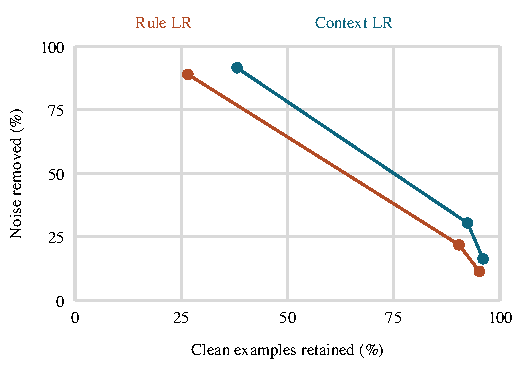
\includegraphics[width=\columnwidth]{tradeoffs.pdf}
\caption{Three development-selected operating points on the main diagnostic. Connecting lines are visual guides, not interpolated deployment policies.}
\end{figure}
\subsection{Robustness and Failure Analysis}

On the 2,735 main test examples with neither a development sentence nor a development entity pair, the context model retains 94.04\% of clean examples and removes 32.87\% of noise. Rule-feature LR retains 90.40\% and removes 18.22\%. This sensitivity analysis reduces one source of overlap; it does not establish generalization to another corpus or resolve prior human exposure to the test set.

\begin{table*}[t]\centering\small
\resizebox{\textwidth}{!}{\begin{tabular}{@{}lrrr@{}}\toprule
Main test subgroup & Model & Clean retained & Noise removed\\\midrule
NA & Rule-feature LR & 90.70 & 24.73\\
NA & Rules + context + relation LR & 93.19 & 28.36\\
non-NA & Rule-feature LR & 89.31 & 12.77\\
non-NA & Rules + context + relation LR & 89.85 & 37.02\\
\bottomrule\end{tabular}}
\caption{Results by candidate-label group on the main diagnostic.}
\end{table*}

The small noise-focused diagnostic has a different composition: 183 of its 297 eligible non-overlapping examples are labeled noise, compared with 979 of 3,966 in the main diagnostic. It also loses many examples under strict span validation. We report it as a separate stress case, not as a directly comparable ARNOR benchmark reproduction.

\begin{table*}[t]\centering\small
\resizebox{\textwidth}{!}{\begin{tabular}{@{}lrrrr@{}}\toprule
Noise-focused method & Clean retained & Noise removed & Noise F1 & ROC AUC\\\midrule
Hand-weighted rules & 91.23 & 39.34 & 54.34 & 0.494\\
Rule-feature LR & 88.60 & 41.53 & 55.88 & 0.788\\
Context + relation LR & 90.35 & 36.07 & 50.77 & 0.654\\
Rules + context + relation LR & 91.23 & 33.88 & 48.63 & 0.664\\
\bottomrule\end{tabular}}
\caption{Noise-focused diagnostic under Retain90. F1 measures noise detection.}
\end{table*}

The context model is weaker than rule-feature LR on this stress case: 33.88\% versus 41.53\% noise recall. Its AUC is also lower (0.664 versus 0.788). A plausible explanation is that the lexical features fit the development distribution better than this selected noise set, but this experiment does not isolate the cause. No architecture or threshold was retuned after seeing these outcomes.

\subsection{Computational Footprint}

\begin{table}[t]\centering\small
\begin{tabular}{@{}lrr@{}}\toprule
Model & Seconds & JSON bytes\\\midrule
Rule-feature LR & 0.154 & 1,042\\
Context + rules LR & 0.255 & 4,093,035\\
\bottomrule\end{tabular}
\caption{CPU scoring on 4,050 valid examples, excluding file input and output.}\label{tab:cpu}
\end{table}

Table 7 summarizes runtime and model size. Timing includes feature extraction, portable JSON scoring, and decisions on 4,050 validated examples. It excludes file IO. There was one warm-up and four measured repeats, with one numerical-library thread requested. These local CPU measurements do not support a speedup ratio against BERT or ARNOR. Model coefficients are plain JSON rather than executable pickle. Invalid spans generate abstentions in the inference CLI.



\section{Discussion and Limitations}

The experiments support a bounded conclusion: relation-conditioned local context improves this lightweight validity filter on the development evaluation and the main diagnostic. The progression from hand-written linguistic hypotheses to learned coefficients and local lexical evidence separates representation quality from operating-point selection. The context-only ablation suggests that lexical features explain most of the additional gain; the noise-focused diagnostic shows that the improvement is distribution-dependent. This release establishes a reproducible supervised sparse baseline, not state-of-the-art performance.

Limitations: the labeled development set is small, many rare relations have very few examples, ambiguous spans are excluded, outer-fold retention fluctuates, and the corpus has been inspected before. Confidence intervals are conditional, the probabilities are not externally calibrated, and choosing a model from development OOF results adds selection uncertainty. The context-only ablation weakens any claim that handcrafted rules are essential. The specialized noise set reveals distribution sensitivity.

The next validation should be fixed before obtaining new results: independently annotate a fresh sentence-grouped holdout; examine rare-relation and domain shift; compare downstream relation extractors trained on all data, filtered data, and matched-size random subsets; and evaluate abstention/review and probability calibration. No downstream gains or neural comparisons are claimed in this release.

\section{Conclusion}
Learning relation-conditioned local context improves the measured noise-removal and clean-retention trade-off over rule-feature logistic regression on grouped development evaluation and the main diagnostic. The context-only ablation and the weaker noise-focused results delimit that conclusion. Fresh annotations and controlled downstream experiments are needed to establish broader utility.
\section*{Contributions and Reproducibility}
The project originated with Zijun Wu, Tianchen Xie, and Tianluo Zhang in Professor Adam Meyers's NLP course. The initial design was discussed jointly; Wu proposed linguistic scoring rules, and teammates contributed tuning and experiments. Coding-agent assistance supported implementation, evaluation, and manuscript preparation. Detailed attribution is documented in the repository.

Code, protocols, models, predictions, and verification scripts are available at \url{https://github.com/JonathanWu04/interpretable-relation-denoising}. Tests cover label leakage, grouped folds, entity masking, thresholds, export parity, and ambiguous records. Raw news text is not redistributed.

\bibliography{references}
\end{document}